\newpage

\section{Materiali ceramici}

Le ceramiche sono materiali inorganici costituiti da metalli o non-metalli. Riconosciamo essenzialmente tre tipologie di ceramiche:

\begin{itemize}
    \item \textbf{\textit{Ceramiche tradizionali}} contenenti argilla (permette la lavorazione), silice (componente refrattario) e feldspato (è una fase fine che si disperde e funge da legante).
    \item \textbf{\textit{Vetri inorganici}} basati sul silicio e raffreddati senza permette la cristallizzazione.
    \item \textbf{\textit{Ceramiche avanzate}} basata su ossidi, carburi e nitruri.
\end{itemize}

I ceramici sono materiali duri e fragili, con valori molto bassi di duttilità, bassa resistenza e tenacità; queste proprietà sono però modulate dalla classe specifica e dalla natura del legame chimico. A seconda della composizione chimica i ceramici presentano legami covalenti (nel caso di composti omopolari come grafite e diamante) che hanno un elevata direzionalità, oppure da legami ionici che non presentano una vera direzionalità \textcolor{red}{EH?}. La maggior parte dei composti ionici presenta anche un certo carattere covalente in funzione dell'elettronegatività.

I materiali ceramici essendo molto vari tra di loro trovano impiego in vari campi. In generale presentano una densità maggiore dell'acqua ma minore dei metalli (2-4 g/cm$^3$), sono resistenti in compressione con un modulo dell'ordine di 1000 MPa (5000 per il diamante) ma sono deboli in trazione con un valore dai 5 ai 10 volte minore (vedi tab. \ref{tab:ceramic_properties}); questo è sopratutto causato da difetti ed imperfezioni alla superficie ed all'interno del cristallo (ad esempio dei vuoti nel campione) che limitano le proprietà meccaniche di questi materiali. Il modulo di Young e la T$_m$ dipendono molto dalla struttura cristallina; il più delle volte T$_m$ non permette di lavorare questi materiali per fusione e vengono usati come materiali refrattari, inoltre hanno anche un basso coefficiente di espansione termica. Inoltre presentano valori di durezza incredibilmente elevati permettendo il loro impiego come abrasivi. Di seguito sono riportati alcuni valori di proprietà meccaniche di qualche materiale ceramico:

\begin{table}[h]
\centering
\begin{tabular}{lccc}
\hline
\textbf{Material}     & \textbf{Traction (MPa)} & \textbf{Compression (MPa)} & \textbf{Elastic Modulus (GPa)} \\ \hline
Allumina               & 200 - 400                          & 2000 - 4000                          & 300 - 400                       \\ \hline
Zirconia              & 200 - 1000                         & 1000 - 2000                          & 200 - 400                       \\ \hline
Silicon Carbide       & 300 - 600                          & 2000 - 4000                          & 400 - 500                       \\ \hline
Silicon Nitride       & 500 - 1000                         & 2000 - 5000                          & 200 - 320                       \\ \hline
Boron Nitride         & 100 - 300                          & 100 - 500                            & 100 - 400                       \\ \hline
\end{tabular}
\caption{Traction, compression strength and elastic modulus of ceramic materials}
\label{tab:ceramic_properties}
\end{table}

Le ceramiche sono caratterizzate da un comportamento fragile che dipende molto dalla presenza di difetti interni e di superficie, trovano dunque impiego strutturale se usati se devono resistere a carichi di compressione. La dipendenza da difetti interni è direttamente collegata al processo di produzione ed anche alla natura stessa del composto, dunque ogni campione presenta delle differenze strutturali interne (che possono essere particolarmente importanti tra due campioni diversi) e pertanto i vari test di trazione non danno un valore preciso ma piuttosto un range. Per migliorare la capacità in trazione difatti si operano processi per creare stati di compressione.
Il metodo di produzione determina anche la porosità del materiale; spesso i ceramici vengono prodotti a partire da polveri. La porosità nel materiale ha un effetto deleterio sulle proprietà meccaniche del nostro materiale (sia sulla rigidezza che sulla resistenza). Si può arrivare a perdere anche il 50\% in resistenza a causa di una porosità del 10\%:
\begin{equation}
    \sigma_{fs}=\sigma_0\exp(-nP)
\end{equation}
Dove $\sigma_{fs}$ è la resistenza alla flessione ed $n$ una costante sperimentale. Altro elemento da tenere in conto è la dimensione del campione: dimensioni maggiori implicano possibilità maggiori di avere cricche all'intero del materiale.

\subsection{Struttura dei ceramici}

La struttura dei cristalli dipende principalmente dal rapporto dei raggi delle specie presenti nel reticolo cristallino. In generale gli anioni sono più grandi dei cationi e questi ultimi andranno ad occupare le posizioni interstiziali del cristallo. 
Se il rapporto tende ad 1 si avrà numero di coordinazione 8 ed il catione si troverà al centro del cubo come nel caso del CsCl. Nel caso di ZnS (zincoblenda) invece lo zinco occupa i siti tetraedrici (la metà per rispettare le corrette proporzioni) all'interno di una cella FCC di zolfo. Il più facile è NaCl con una coordinazione ottaedrica. In generale esistono tanti sali e quindi tante possibili forme diverse. Altre strutture più esotiche ma comunque importanti ed abbondanti sono le perovskiti e gli spinelli.
I materiali ceramici non sono necessariamente cristalli ma possono essere anche solidi amorfi, come il vetro, in cui la silice non ha un pattern periodico ma è disposto in maniera casuale; occorre specificare che la silice presenta anche forme cristalline (Fig \ref{silice}) di vario tipo con la struttura che si organizza con tetraedri di SiO$_4^{4-}$ e può formare anche pattern piuttosto complicati.

\begin{figure}[h]
    \centering
    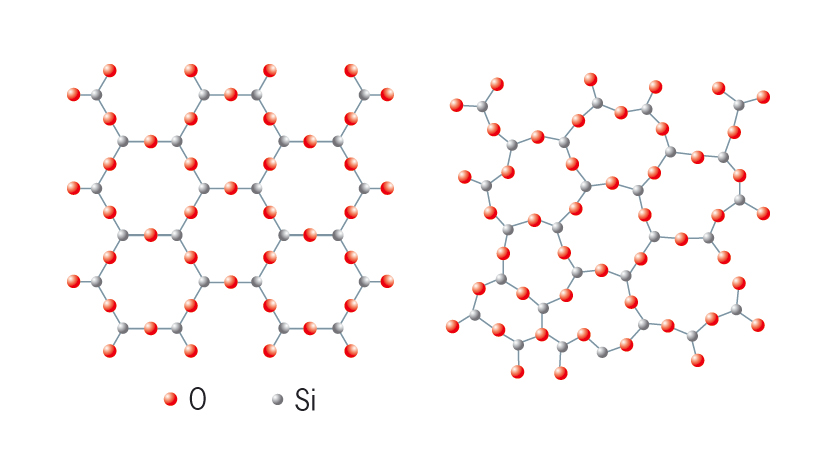
\includegraphics[width=8cm]{ceramici/silice.jpg}
    \caption{Silice amorfa e silice cristallina}
    \label{silice}
\end{figure}

I ceramici cristallini inoltre non presentano dislocazioni: infatti in un solido ionico lo scorrimento degli atomi è quasi impedito, dato che porterebbe alla rottura quasi certa per i composti ionici (lo scorrimento di due filari di atomi porterebbe ioni di segno opposto vicini tra loro, favorendo la rottura del campione); per i covalenti è invece possibile, ma si ha comunque elevata direzionalità. Nel caso di solidi amorfi, non avendo una struttura regolare, non si parla di dislocazione ma piuttosto di processi di tipo viscoso.

\subsection{Ceramiche avanzate}

I ceramici avanzati sono molto duri e spesso vengono impiegati nella produzione di utensili inoltre spesso presentano una tenacità maggiore rispetto ad altri materiali ceramici
\begin{itemize}
    \item Allumina: è utilizzato nei sistemi in cui occorre operare ad alta T mantenendo elevata resistenza meccanica, Trova impiego anche in molti alti campi a causa delle sue proprietà isolanti, abrasive e refrattarie.
    \item Zirconia: è utilizzata come materiale refrattario o aggiunto in altri materiali ceramici. Ha applicazioni simili all'allumina. Presenta diverse transizioni di fase aumentando la T: da tetragonale$\rightarrow$monoclina(1200)$\rightarrow$cubica(2400) fino a fusione (2700). Si può ottenere una forma di zirconia tenacizzata stabilizzando la forma cristallina cubica aggiungendo ossidi al reticolo.
    \item SiC: principalmente usato a causa del suo alto T$_m$ e delle sue sue resistenze a ossidazione ad alta T (maggiori del T di fusione dell'acciaio). è usato come ricopertura nei compositi di Carbonio-Carbonio, è usato anche come abrasivo o come refrattario. L'applicazione più interessante è sicuramente quella da semiconduttore anche ad alta temperatura.
    \item Si$_3$N$_4$ proprietà simili al SiC ma le sua resistenza all'ossidazione alte temperature è leggermente minore. Si prepara insufflando N$_2$ direttamente su Si
    \item Diamante: è usato, oltre che in gioielleria, come abrasivo o come rivestimento per altri materiali.
    \item Silice (SiO$_2$): è l'ingrediente principale del vetro, è possibile creare abrasivi, usarlo come refrattario o come isolante. Può essere anche usato per creare fibre.
    \item TiO$_2$: spesso è usato come pigmento bianco per le superfici o come rivestimento per le medicine. Viene impiegato anche nella protezione di raggi UV.
\end{itemize}

\subsection{Lavorazione}

\begin{itemize}
    \item Sintesi (CVD, decomposizione termica  metodi in soluzione) o estrazione.
    \item Macinazione e mescolamento in acqua o a secco. 
\end{itemize}
Si usano diversi metodi per la sintesi, molti dei quali richiedono l'uso della pressione:
\begin{itemize}
    \item Pressatura a secco: viene usato per materiali ad uso refrattario e per componentistica per elettronica (è unidirezionale).
    \item Pressatura isostatica: Il processo HIP consiste nel porre un oggetto in un ambiente gassoso ad elevata temperatura e elevata pressione isostatica. Lo stampo in questo caso è ermetico e flessibile (di solito di natura elastomerica). Si può lavorare sia a secco che in presenza di un mezzo come acqua o altri tipi di lubrificanti. Viene usato per produrre mattoni, materiali refrattari ed altri tipi di ceramiche.
    \item Hot pressing: le tecniche viste in precedenza con l'uso anche di temperature elevate che permetto di rendere i nostri materiali molto rigidi e ad elevata densità.
\end{itemize}

\begin{figure}[h]
  \begin{minipage}[b]{0.5\linewidth}
    \centering
    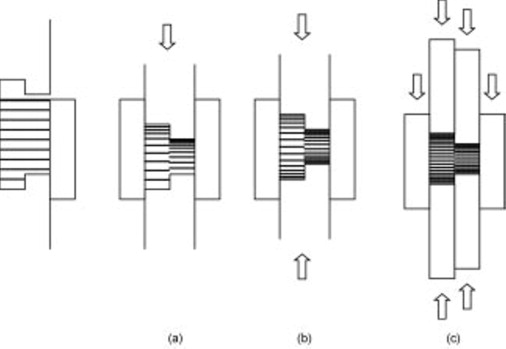
\includegraphics[width=\linewidth]{pressing.jpg}
    \label{pres}
  \end{minipage}
  \begin{minipage}[b]{0.5\linewidth}
    \centering
    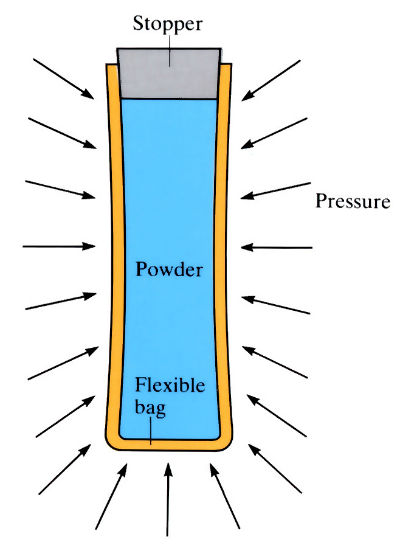
\includegraphics[width=\linewidth]{iso_pressing.jpg}
    \label{iso-pres}  

  \end{minipage}
  \caption{Sinistra: pressatura. Destra, pressatura isostatica}
\end{figure}

Se il materiale lo permetto è anche possibile procedere per fusione a scorrimento (slip casting). Si cola il liquido in un contenitore che assorbe il liquido in cui è contenuto il nostro materiale ceramico. Il materiale in eccesso viene rimosso ed il nostro pezzo viene asciugato e cotto. Anche l'estrusione è un metodo.
I materiali ceramici possono essere sottoposti a diversi trattamenti termici:
\begin{itemize}
    \item Drying or binders removal (si rimuove l'acqua o il solvente organico).
    \item sinterizzazione: pressione+temperatura per avviare processi diffusivi e generare così nuovi oggetti. Una maggiore T di sinterizzazione produce ceramiche con porosità minori
    \item vetrificazione: formazione di una fase vetrosa.
\end{itemize}
Cose sulle fratture e sul fatto che le ceramiche presentano sempre microfratture ed altre cose che ne peggiorano le proprietà. Il fatto che i cristalli possono subire def plastiche solo su particolari piani di scorrimento, in solidi policristallini questa cosa è pressoché impossibile. Pericolosità di fratture superficiali da cui possono espandersi altre cose.
Vetri: silice amorfa e cristallina: vari tipi di additivi: ossidi dei metalli alcalini e ossidi che si integrano nel network: allumina, ossido di titanio e di piombo.
Vari tipi di vetro. Viscosità nei vetri. e produzione vetri. NaCL è FCC ma non è una struttura compatta: gli ioni sulla diagonale non si toccano. CN 12 significa che le dimensioni dell'anione e catione sono uguali. Spinelli, 
Metodi di rafforzamento meccanico e chimico.

\subsection{Ceramici tradizionali}

I materiali ceramici tradizionali sono ottenuti mescolando argilla, silicati e feldspati in varie proporzioni. Il legante è l'acqua che dà luogo ad una serie di reazioni chimiche che modificano le proprietà del materiale. Un vantaggio di questa classe di materiali sono plasticità e malleabilità che permettono al campione di essere lavorato facilmente (\textbf{\textit{idroplasticità}}). La lavorazione può procedere anche per slip casting: una sospensione di argilla o di altro materiale è versata all'interno di uno stampo con le superfici porose in modo tale da avere la deposizione della sospensione. Una volta rimosso il liquido rimane uno strato che per essiccamento diventa solido. In generale questi ceramici richiedono l'essiccamento per rimuovere l'acqua in eccesso, e questo può essere ottenuto lasciando il materiale all'aria oppure riscaldandolo con calore o con IR. Altre volte invece si si può procedere anche alla cottura del pezzo per ottenere proprietà meccaniche differenti. Il materiale a base di argilla ad alte temperature può iniziare a fondersi e creando uno strato di liquido esterno che va a tappare tutte le porosità presenti \textbf{\textit{vitrificazione}}.

\subsection{Vetri}

I vetri sono un'importante categoria di ceramici. Sono principalmente composti da silice amorfa a cui vengono aggiunti vari ossidi (di metalli alcalini o di altri elementi) per modificarne le proprietà chimico-fisiche e renderli adatti a particolari impieghi:
\begin{itemize}
    \item La presenza moderata di B$_2$O$_3$ aumenta la sua resistenza chimica e trova impiego come vetro di laboratorio.
    \item Se in presenza maggiore conferisce al vetro resistenza alle elevate temperature ed allo shock termico e si ottiene il vetro chiamato Pyrex.
    \item Il vetro più impiegato è quello che contiene ossidi di calcio, sodio e magnesio; il principale motivo per cui vengono aggiunti questi ossidi è quello di modificare la composizione chimica del vetro e ridurne la temperatura di fusione.
    \item Vetri ricchi ($>$10\%) di B$_2$O$_3$, Al$_2$O$_3$ e CaO si ottengono dei vetri che possono essere trasformati in fibre (le fibre di vetro appunto).
\end{itemize}
Il grado di cristallizzazione del vetro dipende molto dal rate di raffreddamento e possiede curve simili a quelle di Bain in cui si possono avere fasi vetro-ceramiche se il campione è portato ad opportune temperature; in ogni caso il vetro amorfo è un liquido "super raffreddato" (il grafico del suo volume specifico non presenta una discontinuità a T$_m$ ma un cambio di pendenza a T$_g$).\\
Il vetro può essere rinforzato con la tempra che consiste nel riscaldamento di quest'ultimo rimanendo al di sotto della temperatura alla quale il vetro non riesce più a mantenere la propria struttura senza apparenti deformazioni. I
Il raffreddamento è eseguito lasciando il pezzo caldo all'aria; le superfici del vetro si raffredderanno più velocemente dell'interno mentre l'interno ancora plastico tenderà a contrarsi di più di quanto l'esterno glielo permette (il raffreddamento è seguito da una contrazione, se il raffreddamento è molto veloce la contrazione è minore) creando uno stato di compressione che aumenta la resistenza alla frattura. La forza necessaria a creare la frattura all'esterno deve essere in grado di favorire questa compressione residua. Un altro tipo di tempra è la tempra chimica in cui gli ioni di sodio all'interno del vetro vengono scambiati con del potassio aumentando la resistenza all'impatto, al graffio e alla flessione.
Le ceramiche vetrose trovano largo impiego come materiale dielettrico e per la loro compatibilità biologica.\\
La lavorazione del vetro dipende molto dalla sua viscosità e quindi dalla sua temperatura:
\begin{equation}
    \eta=\eta_0\exp\left(\frac{Q}{RT}\right)
\end{equation}
A temperatura molto elevata la sua viscosità e bassa a sufficienza da permettere la lavorazione. Il raffreddamento può essere critico in quanto lo shock termico può causare la rottura di quest'ultimo.
Un metodo per ottenere un raffreddamento più controllato è l'uso di stagno fuso: alla temperatura di fusione dello stagno il vetro è già solido. La modellazione del vetro invece avviene spesso per stampaggio e per soffiaggio.